\subsection{UCS1 - Importazione dei dati}
\label{sub:ucs1}

%TODO: Add correct image
% Se uno use case esce dalla post allora non mettiamo in scenario secondario ma in estensione
% se invece la post rimane la stessa non è estensione.

\begin{figure}[h]
    \centering
    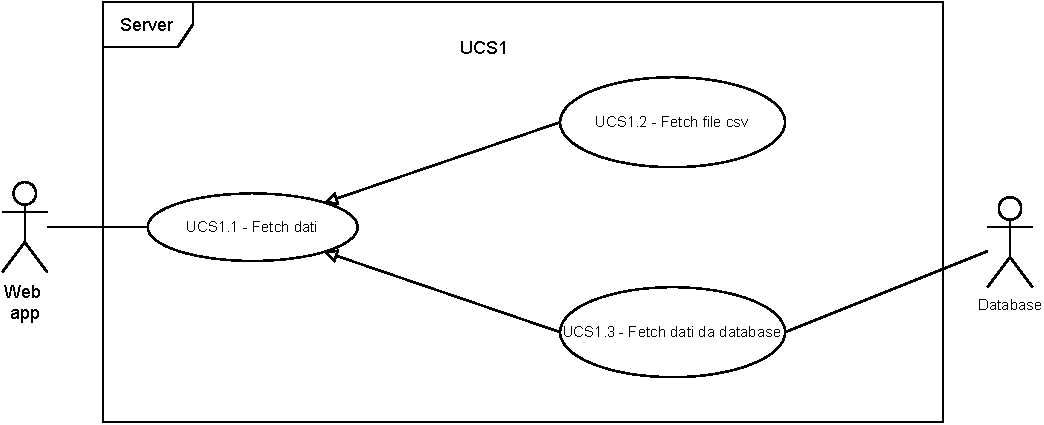
\includegraphics[width=0.7\textwidth]{diagrammi/UCS1.pdf}
    \caption{Diagramma rappresentante UCS1}
    \label{fig:UCS1}
\end{figure}

\begin{itemize}
    \item \textbf{Descrizione}: La Web-App comunica la scelta della fonte dei dati al server che si occupa di importare i dati e di dare automaticamente un metadato di tipo ai campi del dataset.
	
    \item \textbf{Attore primario}: Web-App;
	\item \textbf{Attore secondario}: Database;
        
    \item \textbf{Precondizione}:   L'utente ha selezionato la fonte dei dati (UC1.1);

    \item \textbf{Postcondizione}:  Viene caricato il dataset desiderato dall'utente con i metadati di tipo assegnati o viene visualizzato un messaggio d'errore;

	\item \textbf{Scenario principale}:
		\begin{enumerate}
			\item La web-app comunica al server la decisione dell'utente;
            \item Il server fa il fetch dei dati;
			\item Il server assegna i metadati di tipo
        \end{enumerate}
   
\end{itemize}

\subsubsection{UCS1.1 - Fetch dei dati}

\begin{itemize}

	\item \textbf{Descrizione}: La Web-App comunica la scelta della fonte e il server fa il fetch dei dati.
	
    \item \textbf{Attore primario}: Web-App;
	\item \textbf{Attore secondario}: Database;
        
    \item \textbf{Precondizione}:   L'utente ha selezionato la fonte dei dati (UC1.1);

    \item \textbf{Postcondizione}:  Viene caricato il dataset desiderato dall'utente o viene visualizzato un messaggio d'errore;

	\item \textbf{Scenario principale}:
		\begin{enumerate}
			\item La web-app comunica al server la decisione dell'utente;
            \item Il server fa il fetch dei dati;
        \end{enumerate}
	
\end{itemize}


\subsubsection{UCS1.2 - Fetch dei dati da file csv}

\begin{itemize}

	\item \textbf{Descrizione}: La Web-App comunica la scelta di usare come fonte un file csv e il server fa il fetch dei dati.
	
    \item \textbf{Attore primario}: Web-App;
	        
    \item \textbf{Precondizione}:   L'utente ha selezionato come fonte dei dati un file csv(UC1.2);

    \item \textbf{Postcondizione}:  Viene caricato il dataset desiderato dall'utente o viene visualizzato un messaggio d'errore;

	\item \textbf{Scenario principale}:
		\begin{enumerate}
			\item La web-app comunica al server la decisione dell'utente di usare un file csv;
            \item Il server fa il fetch dei dati;
        \end{enumerate}
		
	\item \textbf{Estensioni}:
		\begin{itemize}
		
			\item Se il file è malformato o vuoto:
			\begin{enumerate}
				
				\item Il caricamento dei dati viene interrotto;
				\item Viene visualizzato un messaggio di errore(UC5)
				
			\end{enumerate}
		
		\end{itemize}
	
\end{itemize}

\begin{figure}[h]
    \centering
    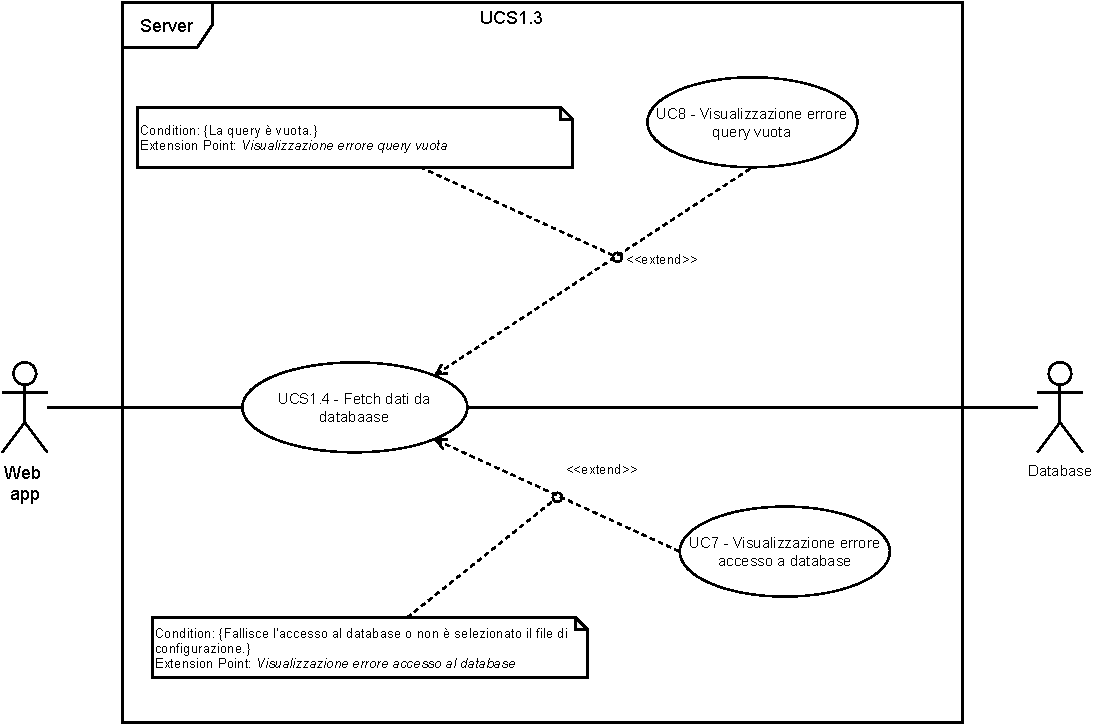
\includegraphics[width=0.7\textwidth]{diagrammi/UCS1_3.pdf}
    \caption{Diagramma rappresentante UCS1}
    \label{fig:UCS1_3}
\end{figure}

\subsubsection{UCS1.3 - Fetch dei dati da database}

\begin{itemize}

	\item \textbf{Descrizione}: La Web-App comunica la scelta di usare come fonte un database e sceglie il file di configurazione adatto. Il server fa il fetch dei dati.
	
    \item \textbf{Attore primario}: Web-App;
	\item \textbf{Attore secondario}: Database;
	        
    \item \textbf{Precondizione}:   L'utente ha selezionato come fonte dei dati un database e ha scelto un file di configurazione(UC1.3);

    \item \textbf{Postcondizione}:  Viene caricato il dataset desiderato dall'utente o viene visualizzato un messaggio d'errore;

	\item \textbf{Scenario principale}:
		\begin{enumerate}
			\item La web-app comunica al server la decisione dell'utente di usare un database e il file di configurazione;
            \item Il server fa il fetch dei dati;
        \end{enumerate}
		
	\item \textbf{Estensioni}:
		\begin{itemize}
		
			\item Se fallisce l'accesso al database:
			\begin{enumerate}
				
				\item Il caricamento dei dati viene interrotto;
				\item Viene visualizzato un messaggio di errore(UC6)
				
			\end{enumerate}
		
			\item Se la query è vuota:
			\begin{enumerate}
				
				\item Il caricamento dei dati non viene effettuato;
				\item Viene visualizzato un messaggio di errore(UC7)
				
			\end{enumerate}
		
		\end{itemize}
			
\end{itemize}